\documentclass[crop,tikz,convert={outext=.svg,command=\unexpanded{pdf2svg \infile\space\outfile}},multi=false]{standalone}[2012/04/13]
%\usetikzlibrary{...}% tikz package already loaded by 'tikz' option
\makeatletter
\usepackage{tikz}
\usepackage{color}
\usetikzlibrary{positioning,shapes.multipart,shapes.geometric, shapes.misc, arrows ,shadows, trees , mindmap, patterns ,tikzmark, calc ,cd, decorations.pathmorphing, intersections, scopes}
\usetikzlibrary{decorations.text}
\usetikzlibrary{decorations.pathreplacing}
\usetikzlibrary{quotes,arrows.meta}
\usepgflibrary {shadings}
\usepackage{fontspec}     
\setmainfont{Lato} 
\begin{document}
	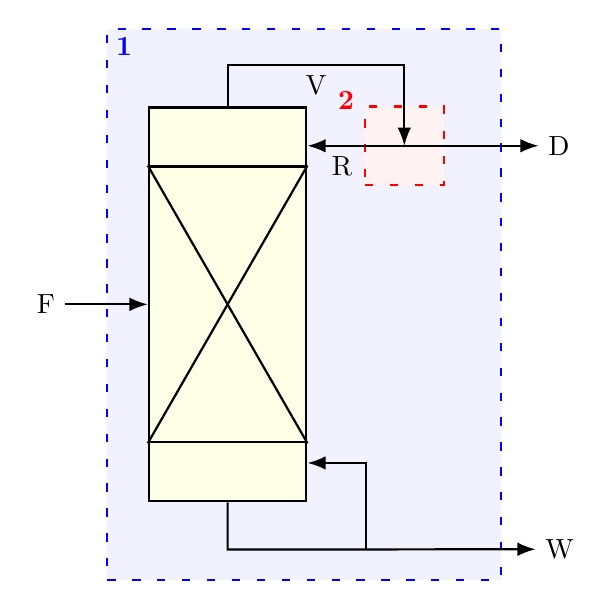
\begin{tikzpicture}
	\node (input) at (0,0)  {F};
	\node [thick, loosely dashed,rectangle, draw=blue!100,fill=blue!5, minimum width=5cm, minimum height=7cm, right = 1.5em of input] (systeem1) {};
	\node [below = 0 em of systeem1.north west,anchor=north west, color = blue!100](sys2){\textbf{1}};
	
	\node [thick,rectangle, draw,fill=yellow!10, minimum width=2cm, minimum height=5cm, right = 3em of input] (box1) {};
	\node [thick,rectangle, draw, minimum width=2cm, minimum height=3.5cm, right = 3em of input] (box2) {};
	\node [thick,rectangle, minimum width=2cm, minimum height=4cm, right = 3em of input] (box3) {};
	
	
	\node [above = 1.5 em of box1](V1){};
	\node [right = 3 em of box3.north east, anchor = center](R1) {};
	\node [right = 5 em of R1](D) {D};
	\node [below = 1 em of box1.south](W1) {};
	\node [right = 5 em of W1.north, anchor = north](W2) {};
	\node [right = 7 em of W2.north, anchor = north](W3) {W};
	
	\node [thick,loosely dashed, rectangle, draw=red!100,fill=red!5,minimum width=1cm, minimum height=1cm, right = 3.5em of box3.north east, anchor = center]  (systeem2) {};
	\node [below = 0.5 em of systeem2.north west,anchor=south east, color = red!100](sys1){\textbf{2}};
	\draw [-Latex, thick] (box1.north) -- (V1.south) -| (systeem2.center)
	node[near start,below]{V};
	\draw [Latex-Latex, thick] (D) -- (box3.north east)
	node[pos=0.85, below]{R};
	\draw [-Latex, thick] (box1.south) -- (W1.south) -- (W3);
	\draw [-Latex, thick] (W2.south) |- (box3.south east);
	\draw [-Latex, thick] (input) -- (box1.west);
	\draw [thick] (box2.north west) -- (box2.south east);
	\draw [thick] (box2.south west) -- (box2.north east);
	\end{tikzpicture}
\end{document}